% file: sections/appendix.tex

\section{附录}

\appendix

%%%%%%%%%%%%%%%
\begin{frame}{实验评估}
  实验目的~\footnotemark[1]~\footnotetext[1]{机器配置: Intel Core i7 3.40GHZ, 4GB RAM.}:
  \begin{enumerate}
    \item 考察 \readcentric{} 算法的实际效率 
      \textcolor{blue}{\small ({\it vs.} 渐近时间复杂度)}
    \item 对比 \readcentric{} 算法与 \rwclosure{} 算法的效率
  \end{enumerate}

  \pause
  \vspace{0.50cm}

  两类负载:
  \begin{enumerate}
    \item 随机生成的系统执行
    \item 满足 \PRAM{} 一致性的系统执行 \textcolor{red}{\small ($\approx$ 最坏情况输入)}
  \end{enumerate}
\end{frame}
%%%%%%%%%%%%%%%

%%%%%%%%%%%%%%%
\begin{frame}{}
  \begin{figure}[t]
    \centering
    \begin{subfigure}[t]{0.50\textwidth}
      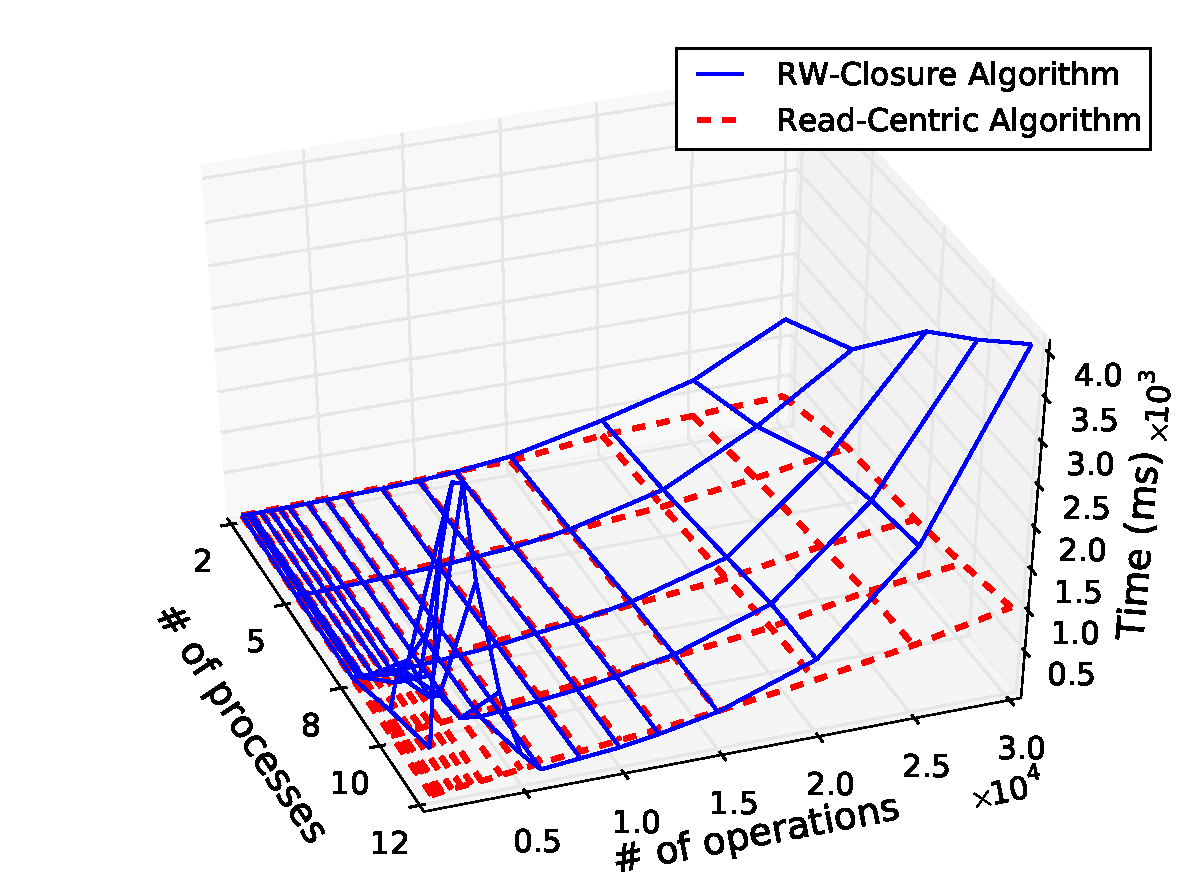
\includegraphics[width = 0.80\textwidth]{figs/vpc-random-cmp.pdf}
    \end{subfigure}%
    ~
    \begin{subfigure}[t]{0.50\textwidth}
      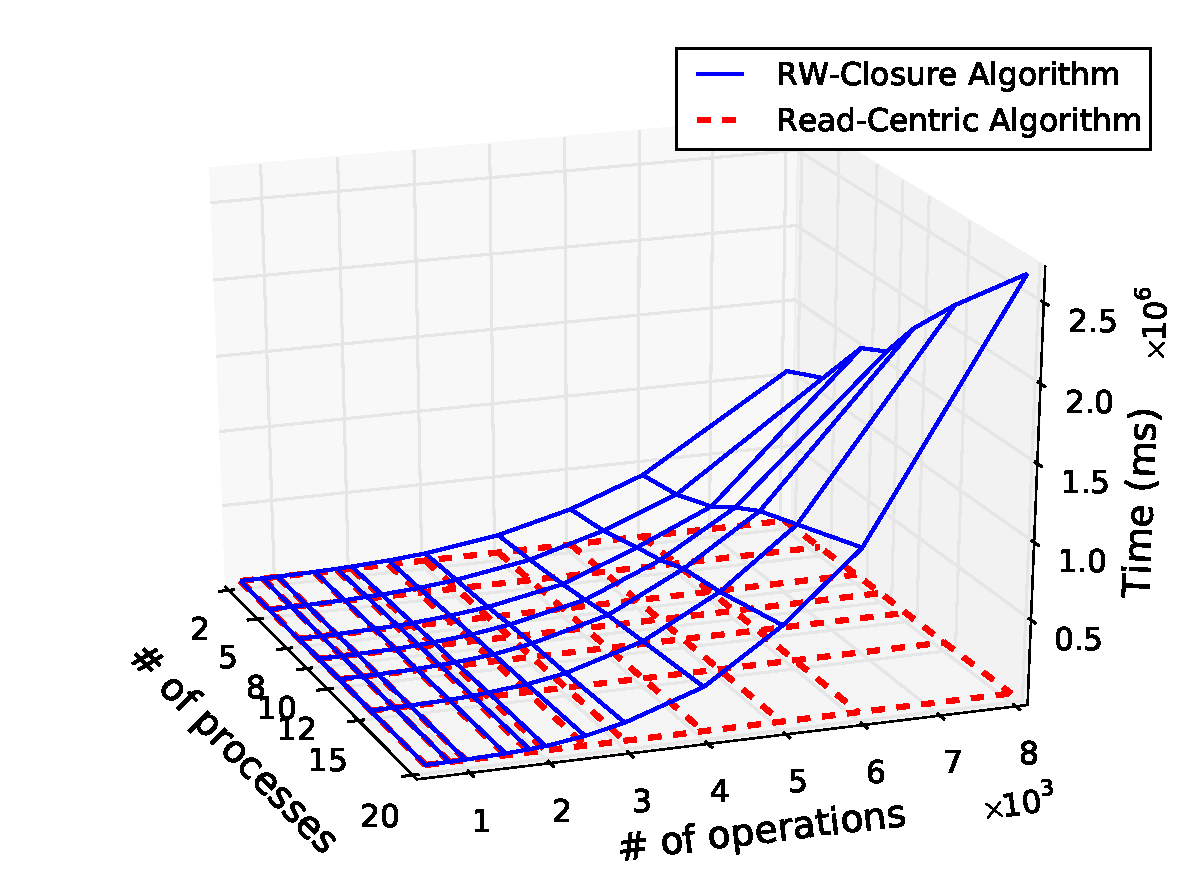
\includegraphics[width = 0.80\textwidth]{figs/vpc-valid-cmp.pdf}
    \end{subfigure}
    \caption{\rwclosure{} 算法与 \readcentric{} 算法在
    \textcolor{blue!80}{ (左) 随机生成}的执行及
    \textcolor{red!80}{ (右) 满足 \PRAM{} 一致性}的执行上的运行时间。}
  \end{figure}

  \pause
  \begin{center}
    \textcolor{red}{(右)} 20个进程、8,000 个操作: 

    \readcentric{} 可获得 694 倍加速.
  \end{center}
\end{frame}
%%%%%%%%%%%%%%%

%%%%%%%%%%%%%%%
\begin{frame}{}
  \fig{width = 0.45\textwidth}{figs/vpc-scalability-more.pdf}
  {\readcentric{} 算法在满足 \PRAM{} 一致性的执行上的运行时间}

  \vspace{-0.30cm}

  \begin{description}
    \centering
    \item[\readcentric{}:] 20个进程、60,000个操作 < 600s~\footnotemark[1]~\footnotetext[1]{用于测试, 规模可用}
    \item[\rwclosure{}:] 20个进程、8,000个操作 > 3,000s
  \end{description}
\end{frame}
%%%%%%%%%%%%%%%
